
\documentclass[sigconf]{acmart}

\usepackage[utf8]{inputenc}
\usepackage{ragged2e}
\setcounter{topnumber}{1}
\graphicspath{ {figures/} }

\newcommand{\Term}[1]{{\bf #1}}

\title{Your title here...}

\author{Joe~Breen}
\affiliation{University of Utah}
\email{joe.breen@utah.edu}
\author{Lincoln~Bryant}
\affiliation{University of Chicago}
\email{lincolnb@uchicago.edu}
\author{Gabriele~Carcassi}
\affiliation{University of Michigan}
\email{carcassi@umich.edu}
\author{Jiahui~Chen}
\affiliation{University of Utah}
\email{jiahui.chen@utah.edu}
\author{Robert W.~Gardner}
\affiliation{University of Chicago}
\email{rwg@uchicago.edu}
\authornote{Corresponding Author}
\author{Ryan~Harden}
\affiliation{University of Chicago}
\email{hardenrm@uchicago.edu}
\author{Martin~Izdimirski}
\affiliation{University of Utah}
\email{nitram.izdi@gmail.com}
\author{Robert~Killen}
\affiliation{University of Michigan}
\email{rkillen@umich.edu}
\author{Ben~Kulbertis}
\affiliation{University of Utah}
\email{ben.kulbertis@utah.edu}
\author{Shawn~McKee}
\affiliation{University of Michigan}
\email{smckee@umich.edu}
\author{Benedikt~Riedel}
\affiliation{University of Chicago}
\email{briedel@uchicago.edu}
\author{Jason~Stidd}
\affiliation{University of Utah}
\email{jason.stidd@utah.edu}
\author{Luan Truong}
\affiliation{University of Utah}
\email{luan.truong@utah.edu}
\author{Ilija~Vukotic}
\affiliation{University of Chicago}
\email{ivukotic@uchicago.edu}

\fancyhead[RE]{J. Breen, et al.}

%% alternatively, the whole team.. probably several more names to add.
%\author{Jiahui~Chen, Martin~Izdmimirski, Ben~Kulbertis, Jason~Stidd, Luan~Trong, Joe~Breen}
%\affiliation{University of Utah}

%\author{Gabriele~Carcassi, Bob~Killen, Shawn~McKee}
%\affiliation{University of Michigan}

%\author{Matt~Henderson}
%\affiliation{New Mexico State University}

%\author{Lincoln~Bryant, Charles~Fraley, Ryan~Harden, Benedikt~Riedel, Ilija~Vukotic, Robert~W.~Gardner}
%\affiliation{University of Chicago}

\begin{abstract}
We describe progress on building the SLATE (Services Layer at the Edge) platform.  The high level goal of SLATE is to facilitate creation of multi-institutional science computing systems by augmenting the canonical Science DMZ pattern with a generic, ``programmable", secure and trusted underlayment platform. This platform permits hosting of advanced container-centric services needed for higher-level capabilities such as data transfer nodes, software and data caches, workflow services and science gateway components. SLATE uses best-of-breed data center virtualization and containerization components, and where available, software defined networking, to enable distributed automation of deployment and service lifecycle management tasks by domain experts. As such it will simplify creation of scalable platforms that connect research teams, institutions and resources to accelerate science while reducing operational costs and development cycle times.
\end{abstract}

\begin{CCSXML}
<ccs2012>
  <concept>
    <concept_id>10010520.10010521.10010537.10010541</concept_id>
    <concept_desc>Computer systems organization~Grid computing</concept_desc>
    <concept_significance>500</concept_significance>
  </concept>
</ccs2012>
\end{CCSXML}
\ccsdesc[500]{Computer systems organization~Grid computing, Edge Computing}


\keywords{Distributed computing, Containerization, Edge computing}

\begin{document}

\copyrightyear{2018}
\acmYear{2018}
\setcopyright{acmcopyright}
\acmConference[PEARC '18]{Practice and Experience in Advanced Research Computing}{July 22--26, 2018}{Pittsburgh, PA, USA}
%\acmBooktitle{PEARC '18: Practice and Experience in Advanced Research Computing, July 22--26, 2018, Pittsburgh, PA, USA}
\acmPrice{15.00}
\acmDOI{10.1145/3219104.3219144}
\acmISBN{978-1-4503-6446-1/18/07}


\maketitle

\section{Motivation}
Multi-institutional research collaborations propel much of the science today.  These collaborations require platforms connecting experiment facilities, computational resources, and data distributed among laboratories, research computing centers, and in some cases commercial cloud providers. The scale of the data and complexity of the science drive this diversity.  In this context, research computing teams strive to empower their universities with emergent technologies which bring new and more powerful computational and data capabilities that foster multi-campus and multi-domain collaborations to accelerate research. Recently, many institutions invested in their campus network infrastructure with these goals in mind. Yet even for the most advanced, well-staffed, and well-equipped campus research computing centers the task is daunting.  Acquiring and maintaining the full scope of cyber-engineering expertise necessary to meet the complex and expanding demands of data and computationally driven science is too costly and does not scale to the full spectrum of science disciplines.  The diversity of computation, data and research modalities all but ensures that scientists spend more time on computation and data management related tasks than on their domain science while research computing staff spend more time integrating domain specific software stacks with limited applicability and sustainability beyond the immediate communities served. Capabilities elsewhere are not available locally, and vice versa.  How should campus and HPC resource providers evolve their cyberinfrastructure to more easily incorporate data infrastructure building blocks developed in other contexts? 

\section{Approach}

We address this challenge in complexity and scaling by introducing a Services Layer At The data center “Edge” (SLATE) which enables distributed automation, centralized delivery and operation of data, software, gateway and workflow infrastructure. Much as Google re-imagined the data center \cite{GoogleDataCenter} and initiated a wave of data center virtualization development, we view advanced “cyberinfrastructure as code” as an appropriate metaphor for transforming the way advanced science platforms are built and operated.  SLATE will augment the Science DMZ pattern \cite{Dart2013} by adding a secure and trusted “underlayment” platform to host advanced data and software services needed for higher-level, connective functions between data centers. These connective services could include, for example, a domain specific content delivery network endpoint, a collaboration data cache, a job (workflow) scheduler, a service component of a distributed science gateway, an http-based software cache, or a resource discovery service (for higher level, meta scheduling systems).

A major focus of SLATE will be development of community accepted Science DMZ patterns capable of supporting advanced and emerging technologies while respecting local site security policies and autonomy. In this project, we are focusing on production services for data mobility, management, and access as driven by data-intensive science domains.  For operators of distributed data management services, content delivery networks, and science gateways SLATE will closely resemble the NIST definition \cite{Mell2011} of a PaaS (Platform-as-a-Service) though the resemblance does not limit the underlying infrastructure to a cloud context.  We are leveraging experience and lessons learned in the deployment and operation of data systems linking over 60 data centers for the LHC computing grid. Figure \ref{fig:slate_vision} gives a schematic of the SLATE concept in the local HPC context.

\begin{figure}
    \centering
    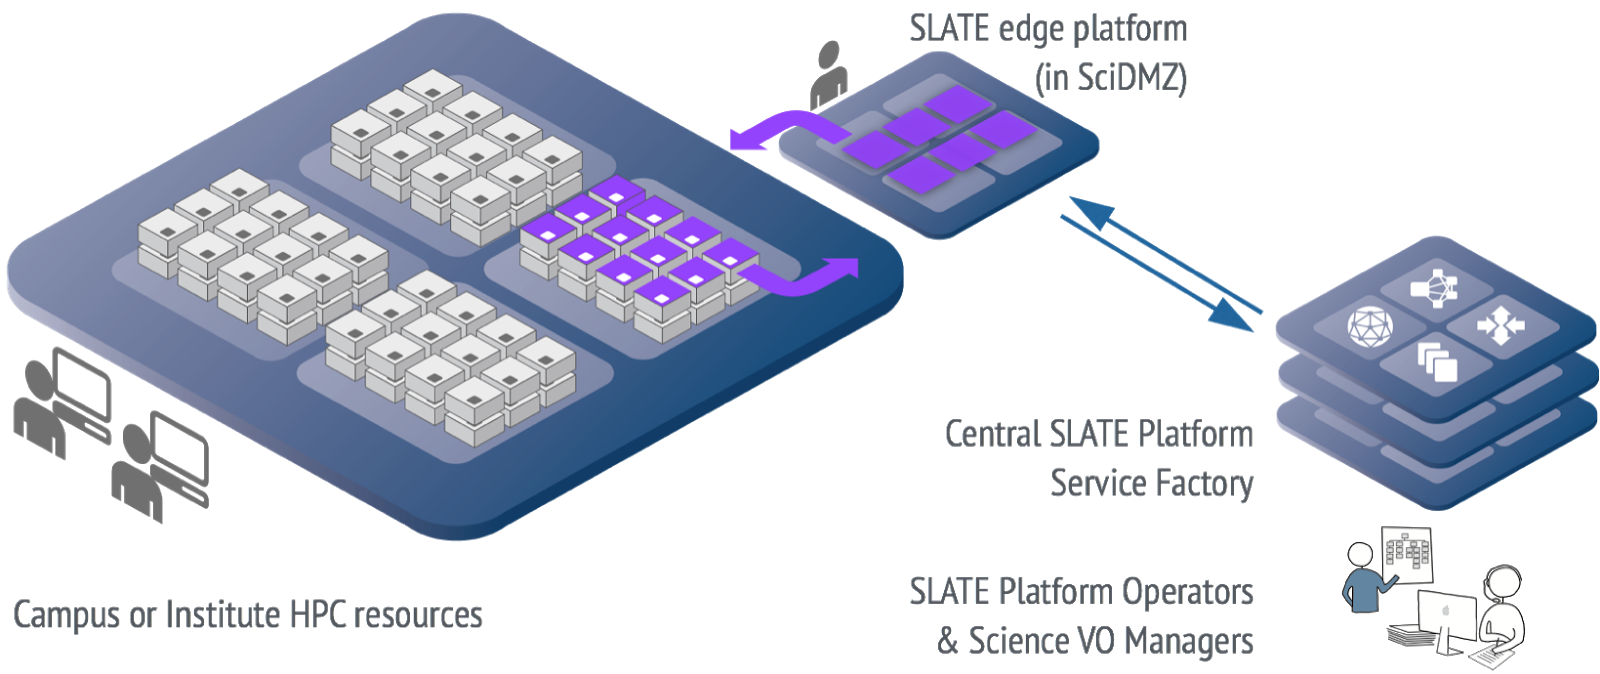
\includegraphics[width=8cm]{slate_vision.png}
    \caption{SLATE implemented in the local HPC context}
    \label{fig:slate_vision}
\end{figure}

The SLATE concept should accommodate large, well-equipped HPC centers, research computing facilities at institutions with fewer resources, as well as  commercial cloud providers.  Modern HPC centers which support data intensive science typically have a Science DMZ which hosts dedicated data transfer nodes, perfSONAR \cite{perfSONAR,perfSONAR_Publications} measurement hosts, and security and enforcement policies needed for high performance, wide area applications.  A dedicated SLATE edge cluster will augment the existing Science DMZ by offering a platform capable of hosting advanced, centrally managed research computing edge services including, where the local infrastructure permits it, the deployment of virtual circuits and other software defined networking constructs \cite{GENI_Stitching,McKeown2008}.  For a small institution with limited resources, the SLATE concept may provide a complete Science DMZ infrastructure to more quickly integrate these institutions into centrally managed research platforms.  The SLATE concept will allow local resource administrators the ability to simply install the infrastructure while offering central research groups the services needed for mdanagement of software and science tools used on the platform.  Thus, a local researcher in a small institution could focus on the science and connecting any requisite science instrumentation, while the local IT staff would not have the burden of trying to understand the science requirements, application software dependencies, data and workflow particulars, etc. A good science use-case comes from a medium sized collaboration to detect dark matter.

\subsection{A Platform for Dark Matter Searches}
Observations of the cosmic microwave background fluctuation, large-scale galaxy surveys, and studies of large-scale structure formation indicate that a large fraction of the matter in the universe is not visible. An exotic but as yet undiscovered elementary particle could explain these observations. Several experiments have been built in last two decades to prove the existence of such elusive particles but their detection has proved challenging as we do not have yet a clear picture of what they are and if they really exist. 

The XENON1T ~\cite{Aprile:2015uzo} experiment, a two-phase xenon Time Projection Chamber has been built in the Laboratori Nazionali del Gran Sasso (LNGS) in Italy to study fundamental questions about the existence and make-up of dark matter.  Commissioning began during the first few months of 2016, with the first large scale science run beginning in December 2016.  Because of its one ton fiducial mass and ultra-low background, the XENON1T experiment is probing properties of dark matter in yet unexplored regions.

A data processing and analysis hub is hosted by the University of Chicago Research Computing Center to complement processing and analysis facilities in Europe (Stockholm is the European analysis hub). A distributed data management service for the collaboration was built so that experiment and simulation data sets at various stages of processing could be distributed and shared easily throughout the 22 member institutes. Figure \ref{fig:xenon_data_management} shows the deployment of the XENON1T Rucio service \cite{Rucio}.  The deployment is a network of five storage endpoints (GridFTP-based data transfer nodes) in Europe and the U.S providing a highly scalable global namespace, a reliable and fast transfer service, a subscription (“placement rules”) service, and a deletion service for data lifecycle management. The raw experimental data are uploaded at the experiment lab and automatically replicated to specific HPC centers for processing, and data products from those systems are registered into the system for distribution to the analysis hubs. The Rucio client tools provide a uniform data access model for the various endpoints.

\begin{figure}
    \centering
    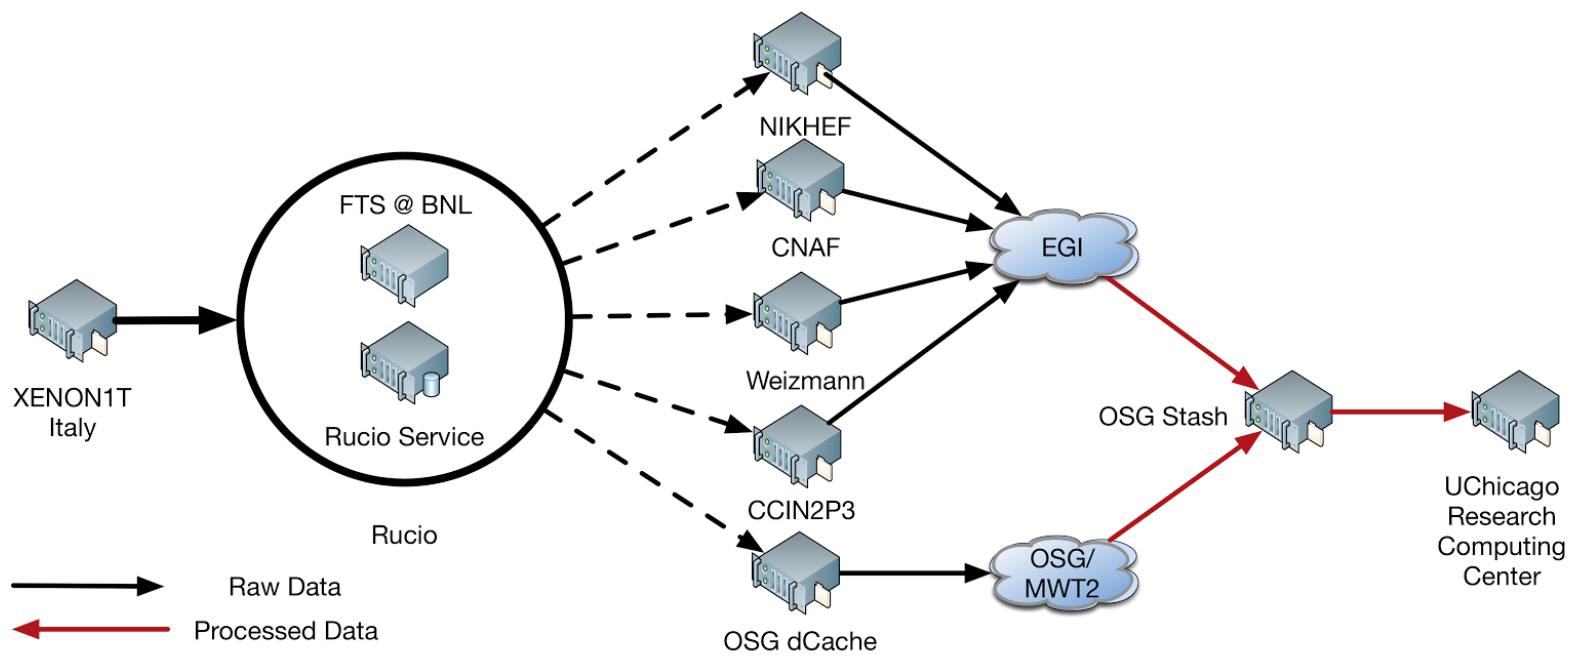
\includegraphics[width=8cm]{xenon_data_management.png}
    \caption{The multi-institution data management platform for the XENON collaboration}
    \justify{\it A central server for managed file transfer is hosted at Brookhaven National Laboratory, and central file and dataset catalogs and service agents are hosted by the University of Chicago. At each of the storage endpoints is a GridFTP service. Each of these services is managed individually so that the platform itself requires efforts from 10 individual administrators. With a SLATE hosted platform, the services, configuration, monitoring and optimization could be managed by a single operator, requiring only basic server management at the endpoints.}
    \label{fig:xenon_data_management}
\end{figure}

We envision the SLATE platform as a key component for scaling and operating data placement services like Rucio for multi-institution science collaborations like XENON1T, especially where local expertise in complex scientific software stacks may be limited.

%\section{Introduction of architecture and concepts}
\section{Architecture}

%\subsection{SLATE Architecture}

SLATE leverages advances made by previous testbeds \cite{Berman2014,GENI,RicciEide:login14,Baldine2012,Chameleon} and similar platforms \cite{Cyverse, PRP} and integrates best-of-breed data center virtualization and service orchestration technologies from the open source community.  The SLATE team has created a platform architecture~\cite{SLATE-Architecture} with a centralized service deployment model in mind. Users coming to the SLATE platform will interact with a centralized API which the SLATE team is is currently developing. This API will have a RESTful design which both the SLATE command line tool and the web portal will use.  The SLATE provisioning service, while firstly targeting the (bare metal) SLATE edge nodes, will have the ability to handle multiple infrastructure types, including various public and private cloud providers.  

The SLATE team has designed the platform to make deployment and operation as streamlined as possible.  Figure~\ref{fig:slate_architecture} gives a schematic picture of the SLATE architecture. The SLATE Platform Portal will provide views for science data operators as well as for operators of the underlying infrastructure at a local institution. 

\begin{figure}
    \centering
    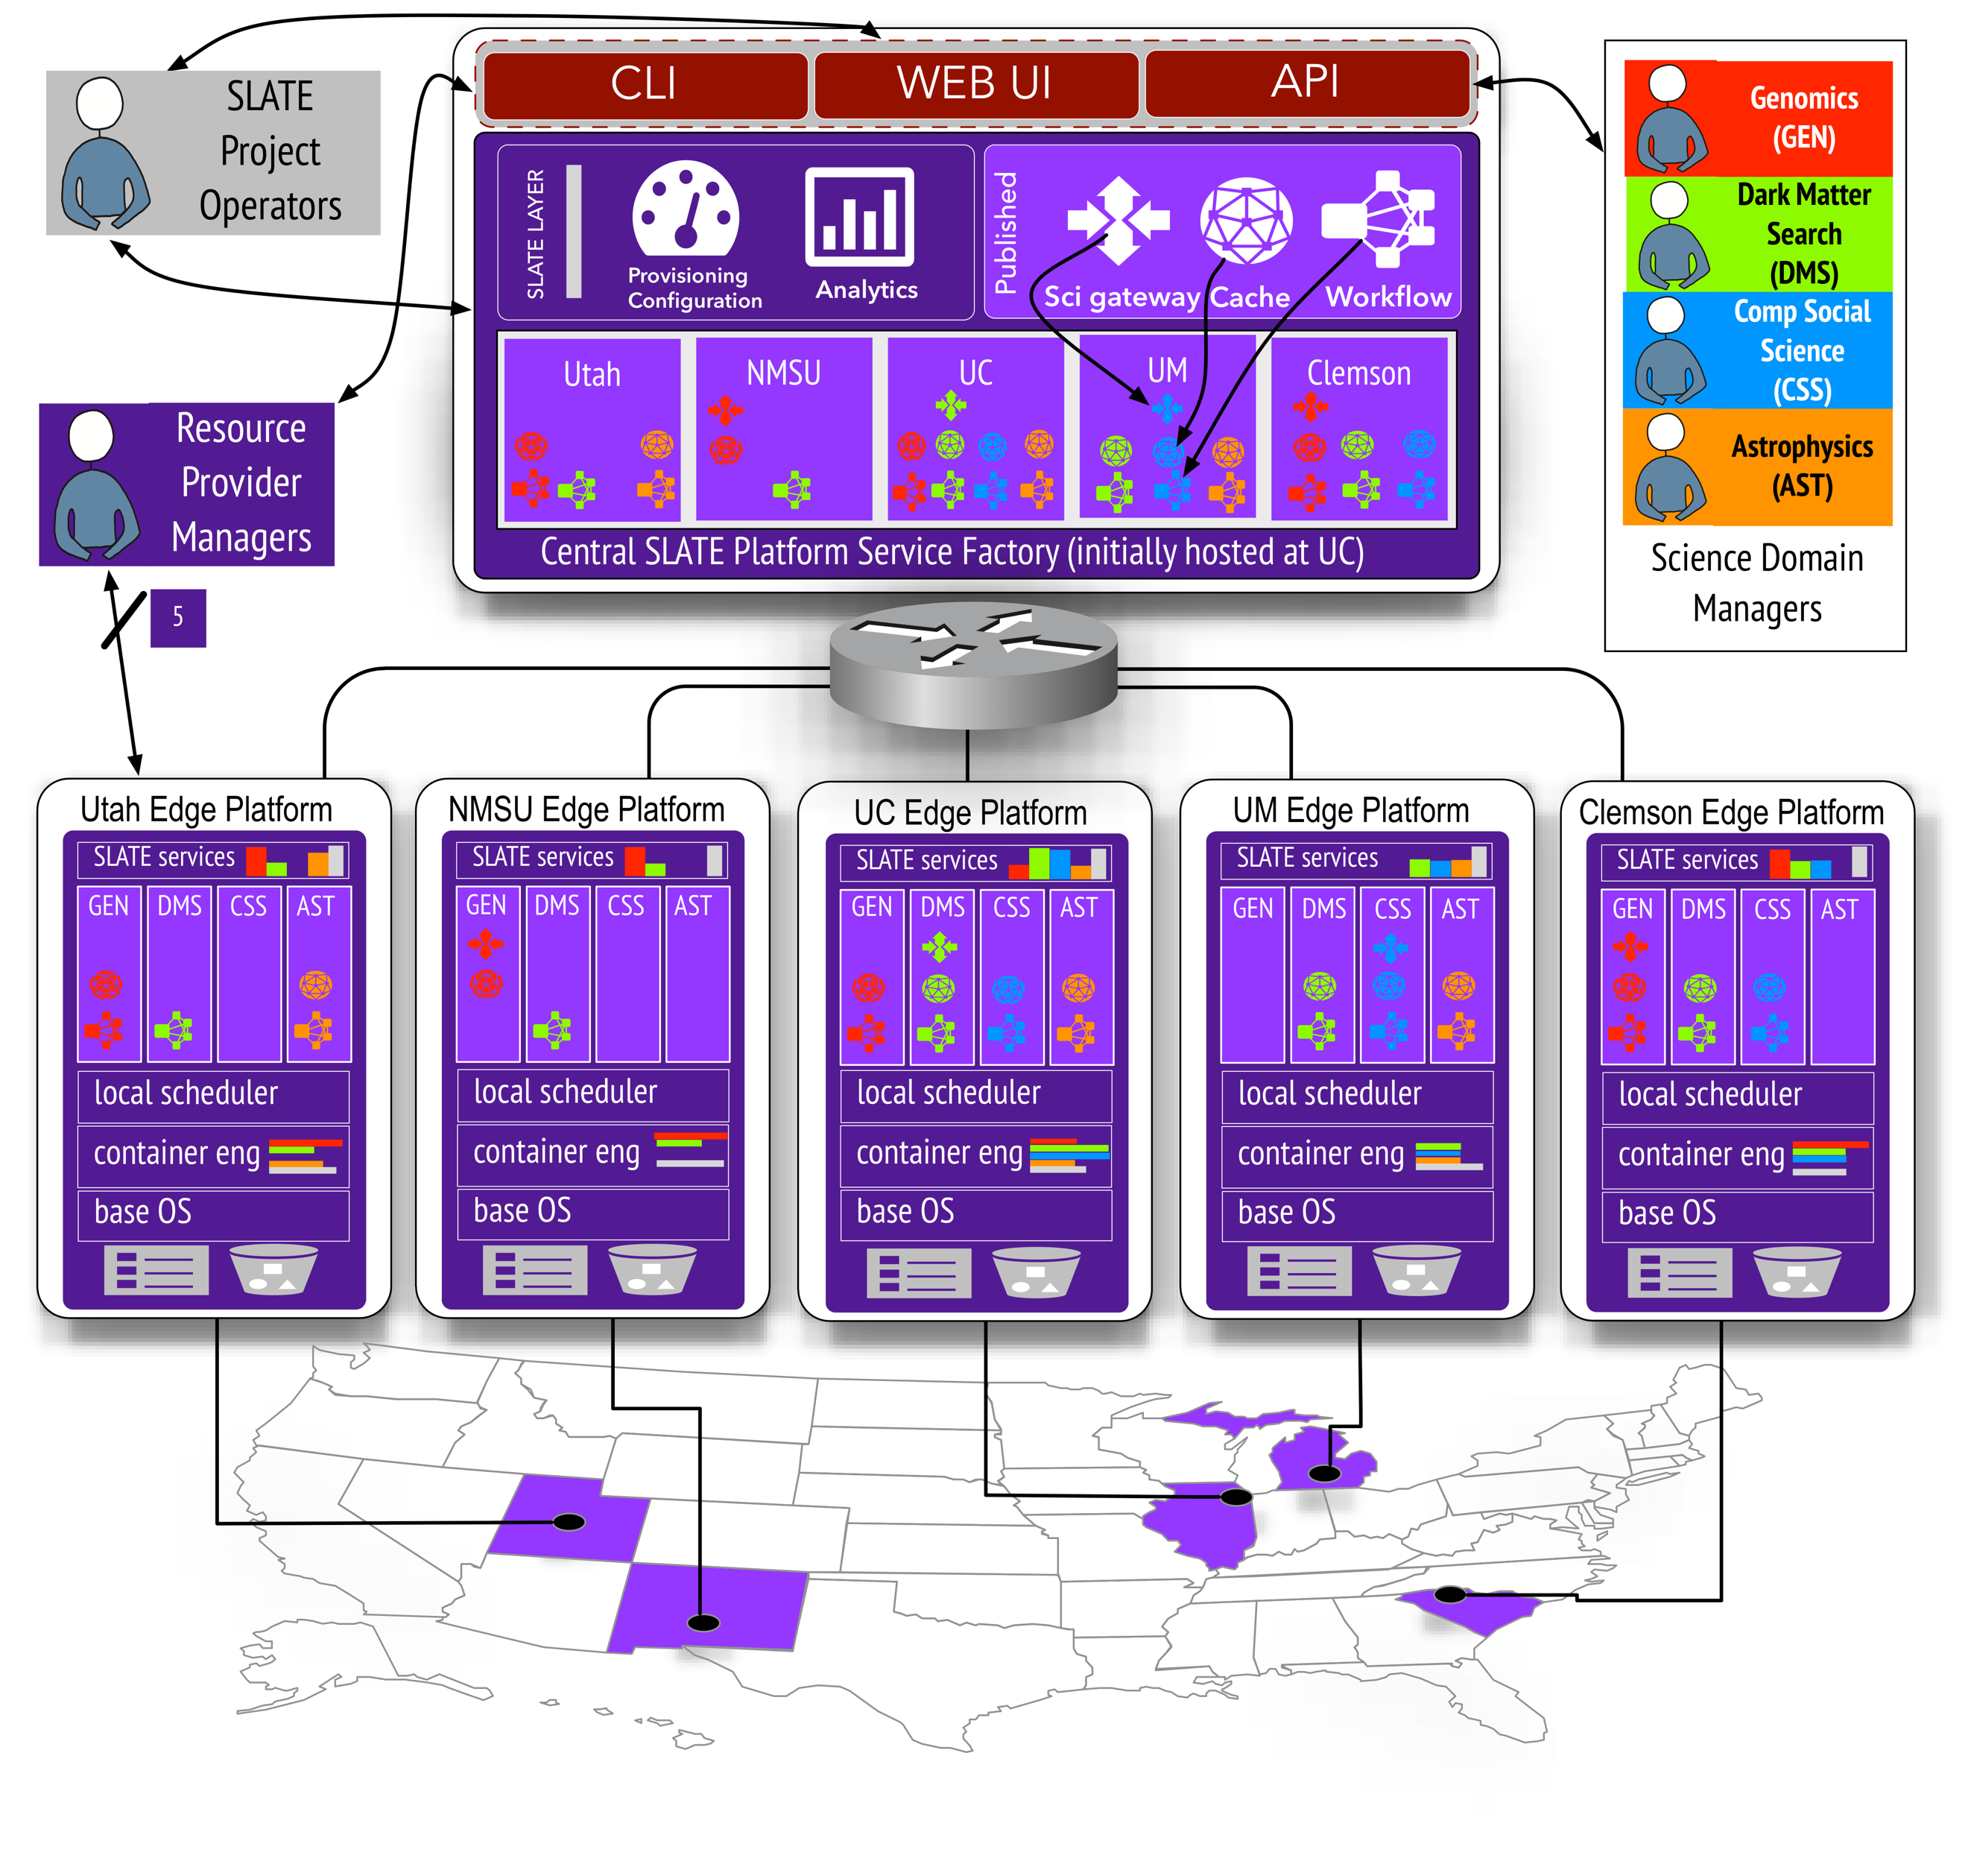
\includegraphics[width=8cm]{slate_architecture.png}
    \caption{SLATE architecture}
    \label{fig:slate_architecture}
\end{figure}


\subsection{Hardware Platform}
The development of the SLATE platform is to facilitate high-throughput, next generation scientific computing applications to interact with both on-premise instruments and facilities, as well as, external upstream services such as those hosted in public clouds or other institutions. One of the key elements of the SLATE platform is a hardware configuration that will minimize the amount of local system administration expertise needed to run complex software stacks, and ideally work as a trusted appliance that lives on the Science DMZ. To that end, we are focusing on three key pieces for the hardware platform deployed at each site:
\begin{itemize}
\item A high performance networking device, either deploying a new device or reusing an existing high performance network device
\item An out-of-band management server, to allow SLATE platform administrators to perform system maintenance and for SLATE central services to stage OS updates and configuration 
\item A scalable compute infrastructure, able to accomodate small sites while allowing for horizontal expansion for larger organizations
\end{itemize}


% I think the vocabulary is implicitly important but I don't think it stands on its own enough to be in the paper. Thoughts? -LB

%\subsection{SLATE Vocabulary}
%
%Understanding context is critical in an environment supporting various virtual services, virtual organizations and resources.  The SLATE Vocabulary document\cite{SLATE-Vocabulary} separates and defines the terms such as SLATE Platform Provider and SLATE Edge Provider for situations when an end site supports multiple SLATE platforms for various organizations.  These terms provide a consistent identification of key concepts, actors and roles within the appropriate context. 

\subsection{Container Orchestration and Federated Services}

In order to realize the vision of deploying and operating edge service applications across disparate resources consistently and at scale, SLATE has adopted a Linux container-based approach to software deployment. This approach, as made popular by Docker and similar products, enables rapid development and deployment by presenting a uniform application environment, and encourages developers to build stateless services for scalability. In the SLATE context, this approach will allow edge service application developers to create services which they can build once and run on any SLATE node.  This approach also simplifies the ability to scale and load balance across resources not only between sites, but across compute platforms within a site as well. 

To facilitate deployments across geographically distributed hardware, the SLATE platform has the capability to federate individual sites. This federation of the individual sites allows scientific edge service application developers to deploy their application at one location and have it replicate across all sites authorized to host the service. Updating an application will follow the same principles, thereby allowing a consistent deployment among all collaborator sites. To facilitate federated applications, the SLATE platform allocates and schedules edge service resources, ensures network connectivity between deployments, configures DNS entries and manages load balancing between sites. In addition, SLATE gives platform and site operators some control over how edge service resources slice and allocate to respective scientific groups sharing the platform. 

%%%% this seems like the Kubernetes implementation specifics are leaking a bit into the abtract description.
%%%% i would hope that whatever system SLATE presents to users would implicitly ensure consistency.
%%%% regarldess I took a stab at addressing that above. -LB

%A key challenge will be the alignment of all the sites so that they may make their resources easily consumable.  Consistent labeling and naming of resources will be critical to enabling the applications to deploy consistently across the federation.  Deployments must be able to make reference to resources by their attributes.  Those attributes must equate to the same values with the same definitions across all member clusters.

%SLATE will provide a set of predetermined namespaces and a predetermined set of labels for all sites. 

\subsection{User-Facing Services and Tools}

In addition to providing a consistent hardware platform and container-based edge service application deployment function, SLATE provides a set of tools to manage the full edge service application lifecycle. This lifecycle includes:
\begin{itemize}
    \item{Application development: taking an existing scientific edge service application and configuring it to run on the SLATE infrastructure}
    \item{Application registration: managing a catalog of edge services that have been approved to be installed on a SLATE platform, either for testing or for general consumption}
    \item{Application usage: taking an application from the catalog, configuration and deploying on the infrastructure}
\end{itemize}

SLATE provides a development environment, which comprises a set of images that can run a virtualized version of a SLATE platform on a development machine. This development environment utilizes technologies such as VirtualBox, minikube, etc., and allows SLATE application developers to work on packaging the application in an isolated environment. 

SLATE also provides an edge service application catalog which the SLATE platform administrator can use to manage the list of applications to install on the SLATE platform.  We use technologies already established in the cloud community such as Kubernetes \cite{Kubernetes1,Kubernetes2}, Helm\cite{Helm} and GitHub\cite{Github}.

As a final piece, SLATE will also need to provide tools to install/monitor/uninstall applications from each SLATE platform. The tools will also need to allow the configuration of the application for the specific use within a science domain.

A good part of the functionality will be provided to the user by interacting to the SLATE service through either a command line interface (CLI), a web user interface (WebUI) or an application programming interface (API). The service will implement the actual logic and expose it through a REST interface which is then consumed by the three different client types. The SLATE service will try to rely as much as possible on the state already provided by the tools it builds upon thus avoiding the problem of synchronize the duplicated state.

\subsection{Edge Service Applications}

A fundamental goal of the SLATE platform is to host edge service applications in support of scientific computing, such as science gateways. The SLATE platform is able to host various services such as data transfer nodes with Globus Connect\cite{GlobusConnect}, caching applications such as Squid\cite{SQUID} and XCache\cite{XCache}, resource sharing applications for job submission and storage sharing, as well as applications used for data organization, delivery and analysis, needed for scalable, multi-institutional collaborations.

All project software running on the SLATE platform will run inside of an application container. This approach allows great flexibility, as experts in a particular domain can provide a specific image for their application. To facilitate allocation and scheduling, all edge service application containers will have to declare a set of resource requirements. These requirements may include disk utilization, minimum throughput (MB/s), firewall ports, memory and CPU.  The SLATE platform will be able to compare these resource declarations to the available resources, and provide a candidate list of resource targets for the application. The platform may go further and suggest changes that could be made to the application for greater proliferation. 

\subsection{Logging and Monitoring}

Though SLATE comprises geographically disparate hardware, the SLATE team maintains central logging and monitoring in order to assess the health of the distributed system.  Centralized monitoring comprises active measurement, i.e. perfSONAR, passive monitoring and log aggregation through tools such as: Check\_mk\cite{checkmk}, Elastic Stack\cite{ElasticStack}, and OSSIM\cite{OSSIM}

\subsection{Security}

The nature of the SLATE platform and its role in providing ``programmable'' access to edge resources makes it critical that we carefully consider all aspects of security in the design and implementation of SLATE.  Sites that deploy SLATE need to be confident that their edge resources will achieve appropriate utilization and will be robust against attacks.  

A key emphasis is that SLATE, by providing a well defined API, enables straightforward vulnerability testing. SLATE provides a specific set of capabilities which external entities can review and analyze in order to help ensure the platform is resilient to attack, and that the platform is following applicable security best practices.  This description is in stark contrast with the situation many sites find themselves when supporting multiple science domains, each with their own unique software stacks and methods. SLATE provides the opportunity to create a specific, well-defined way to interact with a site's resources which a developer can test and validate. 

The SLATE project has scheduled an engagement with the Center for Trusted Scientific Cyberinfastructure (CTSC)\cite{CTSC} and we are already engaging campus security officers to help ensure we are designing a functional and secure cyberinfrastructure component.  This external security discussion is in addition to an internal project-driven focus on providing security as a fundamental design principle in our development, prototyping and testing of SLATE.

\section{Demonstration of Alpha SLATE Distributed Platform}

\subsection{Status of Sites}

As part of its distributed alpha platform, the SLATE team has deployed clusters at three sites: University of Chicago, University of Michigan, and the University of Utah.  For rapid prototyping purposes, the team has deployed these clusters on virtual machines that the team can tear down and re-instantiate at-will. The virtual machines also allow scaling investigation to act as input to the final hardware design.  Currently, we have started architecting the design of the command-line client and will implement a web portal at a later date. 

Since the rapid deployment of science services across multiple sites is a key obective, the SLATE team has been investigating container deployment technologies. While several container orchestration platforms exist, the team is prototyping Kubernetes as an orchestration mechanism based on team members’ initial work, and, based on prevalence in different communities and the market.  
The team has tested Kubernetes on different operating systems such as CentOS, Ubuntu, RancherOS\cite{RancherOS}, and CoreOS\cite{CoreOS}.  The objective of testing the different operating systems was to find a match between what sites use, what sites support, and how to best support and integrate the SLATE platform.  Most HPC environments deploy RedHat or its derivatives (such as CentOS or Scientific Linux) due to the long term stability. However, many Kubernetes deployments run on Ubuntu due to its commercial popularity, more recent kernel, and development tools.  Specific container-focused Linux distributions such as RancherOS and CoreOS have gained popularity due to being relatively light-weight, having customized Kubernetes deployment systems, and custom tooling for update management. 

The alpha configurations at each site chose different operating systems in order to gain some experience with each.  This work has led to an investigation of creating an alpha image on CoreOS as the packaged thrust.  One of the key advantages of CoreOS is the ease of patch management without taking down an entire site for upgrades.  A challenge of CoreOS that the team is still exploring relates to driver support for different hardware, such as GPUs. 

\subsection{SLATE Development Image}

The SLATE team has derived the alpha base image from CoreOS Container Linux, which has a number of features that make it attractive for the SLATE platform. The team can deploy Container Linux as a RAM-resident image, so that containers deploy to disk while the operating system remains ephemeral. For SLATE, this configuration allows for atomic updates via images that can be built and distributed by a centralized upstream system. In the current iteration, a build host with the Container Linux SDK has been prepared, and SLATE-specific changes are pushed to the image at build time. Currently, the team has limited the SLATE-specific changes to installing and configuring a single-node Kubernetes deployment via kubeadm. 

In lieu of forking Container Linux itself, we apply our changes to a base Container Linux image at boot time, using CloudInit \cite{CloudInit}. CloudInit provides a YAML~\cite{YAML}-based configuration language where we define services, configuration files, scripts for fetching binaries from our upstream, etc. Currently, we are deploying the CloudInit configuration as part of the development image, but once we deploy the SLATE hardware platform, we will use a vanilla CoreOS image and apply the SLATE-specific changes at boot. These images and configurations will either stage into, or proxy through, the out-of-band management device. 

\subsection{Initial Federation Testing}

The SLATE alpha federation deployment leverages the Kubernetes Federation project\cite{KubernetesFedProject}.  This project provides two major building blocks:  the ability to sync resources across clusters and the ability to do cross-cluster discovery for DNS and load balancing purposes.  SLATE is primarily leveraging the first building block in order to obtain the ability to present a single point of deployment for an application.  

As part of the initial development work to test the concepts of federation, the SLATE team built a small federation platform for testing. This mini-federation platform allows for initial understanding of the federation technology and quick prototyping of ideas.  The SLATE team has also federated two discrete sites at the University of Michigan and the University of Utah. A small NGINX application has been successfully deployed at the University of Michigan and the University of Utah using the federation tooling. 

%In its initial tests, the SLATE team has deployed simple NGINX applications at the University of Michigan and had those applications deploy at the University of Utah in a consistent fashion.  

% https://github.com/slateci/minifed. not sure if we really need to link this. we'll need to keep it around forever if so.

Testing the current state of federations as provided by Kubernetes has revealed a number of key areas that require work. An initial issue was that some of the tooling that we used to deploy Kubernetes was not sufficiently flexible for federations to work properly. SLATE tooling has taken this issue and other issues into consideration for future deployment iterations. 

Aside from bugs and minor issues in the Kubernetes federation control plane, we found that two key areas were lacking in our tests. First, the federation tooling required that we maintain consistent naming and labeling across multiple sites. This requirement implies that either some upstream contributions will need to integrate into Kubernetes itself, or the SLATE subsystem responsible for site-level configuration will need to ensure the naming and labeling maintains the proper consistency, external to Kubernetes. The second issue is that the federation tooling, as it currently exists, requires a high level of permissions (and therefore trust) between sites and site administrators. This particular issue presents serious security considerations for SLATE deployments across disparate resources. 

%\begin{itemize}
%    \item{Issues with current version of Rancher being too opinionated for federation software to interact %successfully}
%    \item{Issues with maintaining consistent naming and labeling across multiple sites}
%    \item{Issues with the lack of a federated clean-up mechanism due to software bugs}
%    \item{Issues with the high level of permissions required across sites for federation}
%\end{itemize}

%The last challenge is the most significant since current Kubernetes federations require a high level of trust among the disparate site administrators.  A full federation administrator is essentially a cluster administrator on EVERY cluster.

\subsection{Progress of CLI Development}

To expedite the development of the command-line tools and services, we are currently developing the CLI as a single tool with no distinction between frontend and backend. By getting the tool into the hands of developers quickly, this allows us to rapidly iterate upon the semantic definition of the commands we need to provide. However, the current implementation keeps the interface fully separate from the backend logic, such that a client/server model can implement later as the other SLATE platform components develop. 

%%%% This needs to be a bit less negative. -LB
%The development is being carried on in Go, as this is the language used for implementing Kubernetes and related projects. Originally, we envisioned this would allow us to better integrate with their code but unfortunately this has not been the case. The project we have to build upon do not seem to be providing a stable client API and the tools themselves are still under considerable rewriting (e.g. in the next version helm may remove the server side component from their architecture). This, coupled with by Go’s lack of support for standard software engineering practices (e.g. there is no best practice for versioning of dependencies), forces us to adopt a very defensive stance for development which is ultimately sub-optimal. For example, since the command line tools are the only distributed artifact that are versioned, our prototype simply uses shell invocation and output parsing in the hope that this interface will undergo fewer changes.

%%%% better? -LB
We have chosen to develop the command-line tooling in Go\cite{Go}, as this language is the language of choice to develop Kubernetes and related projects in this space, such as Docker\cite{Docker} and etcd\cite{etcd}. One of the challenges we have encountered in developing the SLATE CLI is that many of the underlying tools and components are themselves under heavy development and thus moving very rapidly. While this rapid development is a positive sign that the Kubernetes and associated projects have a healthy and active developer community, this rapid change has forced us to take a conservative stance with regard to how we interface with these tools. Currently, the we have prototyped the following commands:
\begin{verbatim} slate dev start \end{verbatim} 
This command starts the development environment. This environment consists of minikube\cite{Minikube} (which is assumed to be available and properly installed) properly configured with Helm and the SLATE application catalog\cite{Slate-Catalog}.
\begin{verbatim} slate app install \end{verbatim}
This command installs an application from the application catalog.
\begin{verbatim} slate app delete \end{verbatim} 
This command removes already installed applications.
\begin{verbatim} slate dev delete \end{verbatim} 
This command tears down the development environment. Figure \ref{fig:cli_lifecycle} shows an example of the working tool.

\begin{figure}
    \centering
    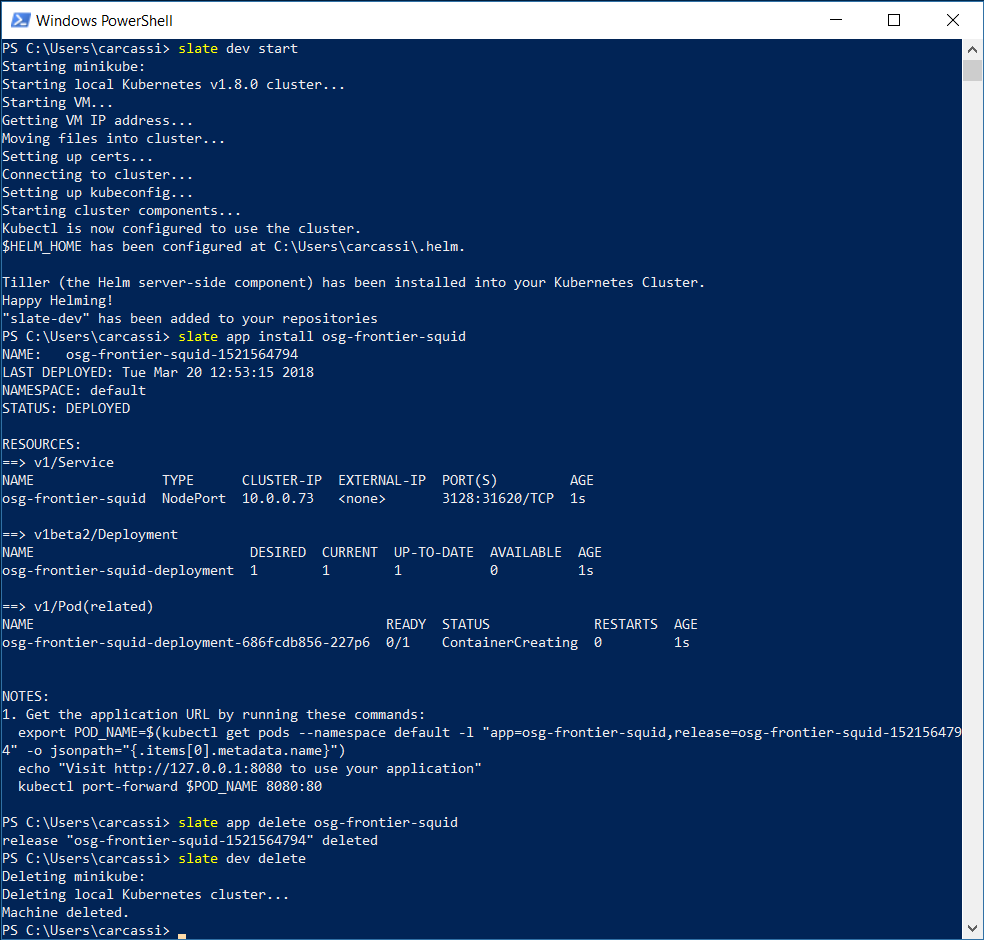
\includegraphics[width=8cm]{commandline_install_lifecycle.png}
    \caption{Example of command line installation lifecycle}
    \label{fig:cli_lifecycle}
\end{figure}

\subsection{Applications}

The SLATE team has deployed several applications on its alpha platform.: JupyterHub, perfSONAR, Elasticsearch, and Kibana.  The team has also created an XCache \cite{XCache} prototype in order to demonstrate caching, an essential feature of future distributed data delivery networks.  

The team is working to prototype a process for packaging these using a combination of SLATE developed tools, Helm and other tools.  The SLATE deployment process will comprise the testing and integration of the application container, as well as the ability to deploy the application container across the federation.
  
The SLATE team has encountered a number of challenges which the team is attempting to mitigate in its packaging and deployment process.  Some of those challenges are:
\begin{itemize}
    \item Library support
    \item Helm support
    \item Package builds focused on virtual machine installations as opposed to containers
    \item Location of static config files for packages so that containers can be ephemeral
\end{itemize}


\subsubsection{XCache deployment}

XCache  is a caching service that can reduce latency and reduce bandwidth needs of the wide area network accesses based on the XRootD \cite{xrootd} protocol. Reliable operation of the XCache service, without local systems administrator input, is very important for the successful utilization of network resources by the experiments at the CERN Large Hadron Collider which must deliver data to hundreds of HPC centers. Resources needed by the application depend on the scale of the computing resources served by the cache and range from a single caching node with 10~Gbps network interface card and a few terabytes  of disk, to a cluster of caching nodes and hundreds of terabytes of disk. The single-node use case is very simple: a single pod with the xrootd server is run, with only one service exposing port 1094. Cluster installation is more complex requiring two services per node (xrootd and cmsd), and a "master" service that unifies them. Client authentication is based on X509\cite{RFC5280} certificates, while the XCache service itself authenticates against data origins (XRootD services at different storage elements) using so-called ``robot" certificates. Figure~\ref{fig:data_lakes} shows a production implementation which uses SLATE as the management layer in the edge network.  A production deployment will have three more services:
\begin{itemize}
    \item Service registration. A health-check probe will automatically register and enable an XCache endpoint in an information service, and blacklist it when necessary.   
    \item Reporting of cache state. In addition to caching blocks of data accessed, XCache stores important metadata per file. This metadata includes: number of accesses, times of first and last access, number of blocks accessed, etc. All this information is periodically aggregated and reported to a central monitoring service. 
    \item Summary stream reporting. Every minute, the service reports important operational parameters of the XCache server, including number of connections, number of errors, memory used, etc. 
\end{itemize} 

XCache is one of the first science applications supported on the SLATE platform, and has driven requirements for the initial alpha platform. The team has packaged XCache for a Kubernetes deployment, including a Dockerfile, Kubernetes YAML files, scripts to create and retrieve shared secrets, etc. All code and configuration lives on Github, and hooks are enabled to automatically build XCache via DockerHub. 

\begin{figure}
    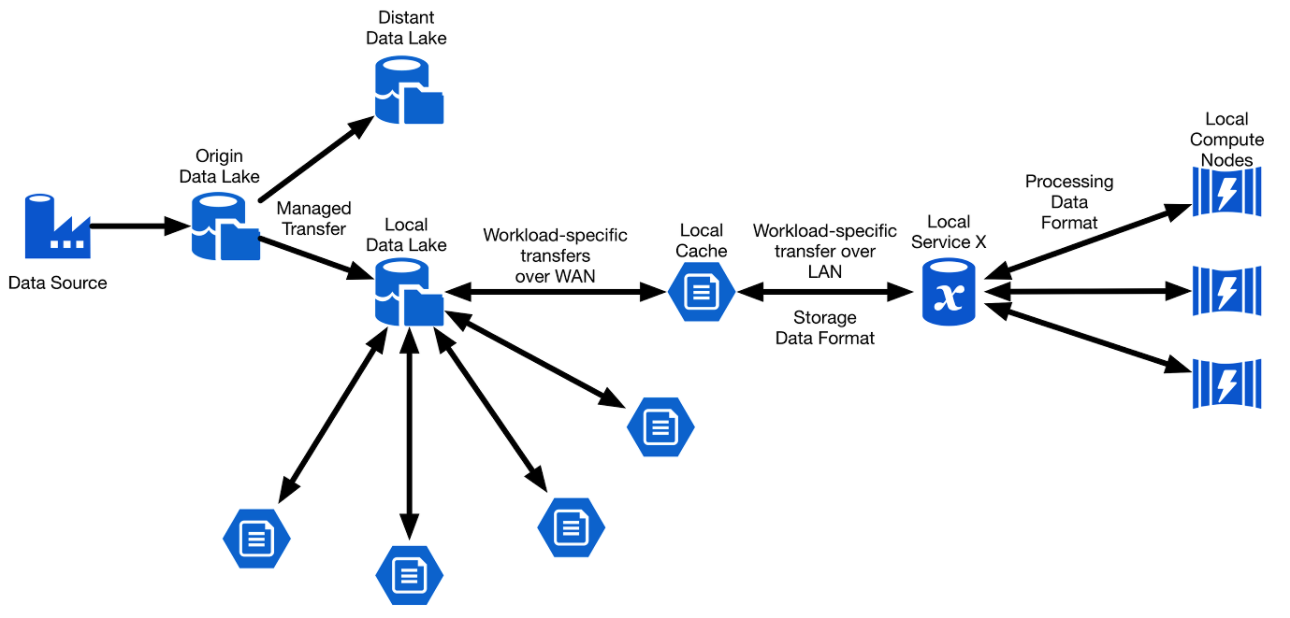
\includegraphics[width=8cm]{data-lake2.png}
    \caption{Example distributed caching and data delivery service  using SLATE}
    \justify{\it A data lake service can deliver experimental data to processing facilities using a network of caching servers and purpose-built delivery services that transform the data into the needed format.}
    \label{fig:data_lakes}
\end{figure}


\subsection{Logging and Monitoring}

Logging and monitoring of a distributed infrastructure requires both a central and distributed approach.  The University of Chicago has deployed a central Elastic Stack\cite{ElasticStack} and Prometheus\cite{Prometheus} for gathering data from the remote sites.  For visualization, Grafana allows for different dashboards and perspectives.  Each site is running perfSONAR and the Elastic Stack to support active measurement and passive collection.  

\section{Summary \& outlook}

The SLATE team has completed a first iteration of its alpha version platform distributed and federated over three sites.  The next iteration in the project will be to harden the packaging of the image, package example applications for deployment, test the loading and scaling of the platform, finalize the hardware configuration based on loading and scaling, and start to explore the network aspects.  The project welcomes contributions and participation from groups and individuals focused on building distributed research platforms and gateway systems. Interested readers may follow developments at http://slateci.io/. 

\section*{Acknowledgements}

This work is supported by the National Science Foundation Office of Advanced Cyberinfrastructure (OAC), grant number 1724821.

\bibliographystyle{acmbibliography}
\bibliography{references}

\end{document}
